% ---------------------------------------------------------------------------------------------------------------
% TEMPLATE PARA TRABALHO DE CONCLUSÃO DE CURSO
% Pontifícia Universidade Católica de Minas Gerais - PUC Minas
% Customização da classe abnTeX2 (http://www.abntex.net.br/) para as normas da PUC Minas
% Baseado na classe abnTeX2 da Universidade Federal Tecnológica do Paraná
% Adaptado para seguir as regras de normalização da PUC Minas <http://portal.pucminas.br/biblioteca/>
%
% Autores da customização original: 
%        Diego Marczal
%        Michael Vornes <https://github.com/mvornes>
%
%----------------------------------------------------------------------------------------------------------------
% Codificação: UTF-8
% LaTeX:  abnTeX2          
% ---------------------------------------------------------------------------------------------------------------


% CARREGA CLASSE PERSONALIZADA DA PUC MINAS--------------------------------------------------------------------------
\documentclass[%twoside,                   % Impressão em frente e verso
    	        oneside,                   % Impressão apenas frente
]{configuracoes/pucminas-abntex2}


% INCLUI ARQUIVOS DE CONFIGURAÇÕES-------------------------------------------------------------------------------
% REFERÊNCIAS------------------------------------------------------------------
\usepackage[%
    alf,
    abnt-emphasize=bf,
    bibjustif,
    recuo=0.0cm,
    abnt-url-package=url,       % Utiliza o pacote url
    abnt-refinfo=yes,           % Utiliza o estilo bibliográfico abnt-refinfo
    abnt-etal-cite=3,
    abnt-etal-list=3,
    abnt-thesis-year=final
]{abntex2cite}                  % Configura as citações bibliográficas conforme a norma ABNT

% PACOTES----------------------------------------------------------------------
\usepackage[utf8]{inputenc}                                 % Codificação do documento
\usepackage[T1]{fontenc}                                    % Seleção de código de fonte
\usepackage{booktabs}                                       % Réguas horizontais em tabelas
\usepackage{color, colortbl}                                % Controle das cores
\usepackage{float}                                          % Necessário para tabelas/figuras em ambiente multi-colunas
\usepackage{graphicx}                                       % Inclusão de gráficos e figuras
\usepackage{icomma}                                         % Uso de vírgulas em expressões matemáticas
\usepackage{indentfirst}                                    % Indenta o primeiro parágrafo de cada seção
\usepackage{microtype}                                      % Melhora a justificação do documento
\usepackage{multirow, array}                                % Permite tabelas com múltiplas linhas e colunas
\usepackage{subeqnarray}                                    % Permite subnumeração de equações
\usepackage{lastpage}                                       % Para encontrar última página do documento
\usepackage{verbatim}                                       % Permite apresentar texto tal como escrito no documento, ainda que sejam comandos Latex
\usepackage{amsfonts, amssymb, amsmath}                     % Fontes e símbolos matemáticos
\usepackage[algoruled, portuguese]{algorithm2e}             % Permite escrever algoritmos em português
\usepackage{pslatex}                                        % Usa a fonte Times New Roman
\usepackage[bottom]{footmisc}                               % Mantém as notas de rodapé sempre na mesma posição
\usepackage{ae, aecompl}                                    % Fontes de alta qualidade
\usepackage{latexsym}                                       % Símbolos matemáticos
\usepackage{lscape}                                         % Permite páginas em modo "paisagem"
%\usepackage{picinpar}                                      % Dispor imagens em parágrafos
%\usepackage{scalefnt}                                      % Permite redimensionar tamanho da fonte
%\usepackage{subfig}                                        % Posicionamento de figuras
%\usepackage{upgreek}                                       % Fonte letras gregas

% CONFIGURAÇÕES DE APARÊNCIA DO PDF FINAL--------------------------------------
\makeatletter
\hypersetup{%
    portuguese,
    colorlinks=true,   % true: "links" coloridos; false: "links" em caixas de texto
    linkcolor=blue,    % Define cor dos "links" internos
    citecolor=blue,    % Define cor dos "links" para as referências bibliográficas
    filecolor=blue,    % Define cor dos "links" para arquivos
    urlcolor=blue,     % Define a cor dos "hiperlinks"
    breaklinks=true,
    pdftitle={\@title},
    pdfauthor={\@author},
    pdfkeywords={abnt, latex, abntex, abntex2}
}
\makeatother

% ALTERA O ASPECTO DA COR AZUL--------------------------------------------------
\definecolor{blue}{RGB}{41,5,195}

% REDEFINIÇÃO DE LABELS---------------------------------------------------------
\renewcommand{\algorithmautorefname}{Algoritmo}
\def\equationautorefname~#1\null{Equa\c c\~ao~(#1)\null}

% CRIA ÍNDICE REMISSIVO---------------------------------------------------------
\makeindex

% HIFENIZAÇÃO DE PALAVRAS QUE NÃO ESTÃO NO DICIONÁRIO---------------------------
\hyphenation{%
    qua-dros-cha-ve
    Kat-sa-gge-los
}



% INCLUI ARQUIVOS DO TRABALHO DE CONCLUSÃO DE CURSO (PRÉ-TEXTUAIS, TEXTUAIS, PÓS-TEXTUAIS)-----------------------

% INSERE CAPA E FOLHA DE ROSTO
% CAPA---------------------------------------------------------------------------------------------------

% ORIENTAÇÕES GERAIS-------------------------------------------------------------------------------------
% Caso algum dos campos não se aplique ao seu trabalho, como por exemplo,
% se não houve coorientador, apenas deixe vazio.
% Exemplos: 
% \coorientador{}
% \departamento{}

% DADOS DO TRABALHO--------------------------------------------------------------------------------------
\titulo{Adoção de plataforma de disponibilização de material científico traduzido: 
	Um análise sobre disposição de pessoas e instituições de ensino superior para 
	colaboração com a distribuição democrática do conhecimento científico}
%\titleabstract{Title in English}
\autor{Elias Flávio de Paiva}
%\autorcitacao{SOBRENOME, Nome} % Sobrenome em maiúsculo
\local{Contagem}
\data{2018}

% NATUREZA DO TRABALHO-----------------------------------------------------------------------------------
% Opções: 
% - Trabalho de Conclusão de Curso (se for Graduação)
% - Dissertação (se for Mestrado)
% - Tese (se for Doutorado)
% - Projeto de Qualificação (se for Mestrado ou Doutorado)
\projeto{Trabalho de Conclusão de Curso}

% TÍTULO ACADÊMICO---------------------------------------------------------------------------------------
% Opções:
% - Bacharel ou Tecnólogo (Se a natureza for Trabalho de Conclusão de Curso)
% - Mestre (Se a natureza for Dissertação)
% - Doutor (Se a natureza for Tese)
% - Mestre ou Doutor (Se a natureza for Projeto de Qualificação)
\tituloAcademico{Bacharel}

% ÁREA DE CONCENTRAÇÃO E LINHA DE PESQUISA---------------------------------------------------------------
% Se a natureza for Trabalho de Conclusão de Curso, deixe ambos os campos vazios
% Se for programa de Pós-graduação, indique a área de concentração e a linha de pesquisa
\areaconcentracao{}
\linhapesquisa{}

% DADOS DA INSTITUIÇÃO-----------------------------------------------------------------------------------
% Se a natureza for Trabalho de Conclusão de Curso, coloque o nome do curso de graduação em "programa"
% Formato para o logo da Instituição: \logoinstituicao{<escala>}{<caminho/nome do arquivo>}
\instituicao{Pontifícia Universidade Católica de Minas Gerais}
\departamento{ICEI - Instituto de Ciências Exatas e Informática}
\programa{Curso de Bacharelado em Sistemas de Informação}
\logoinstituicao{0.2}{dados/figuras/logo-instituicao.png} 

% DADOS DOS ORIENTADORES---------------------------------------------------------------------------------
\orientador{Cleia Marcia Gomes Amaral}
%\orientador[Orientadora:]{Nome da orientadora}
\instOrientador{Pontifícia Universidade Católica de Minas Gerais}

%\coorientador{Nome do coorientador}
%\coorientador[Coorientadora:]{Nome da coorientadora}
%\instCoorientador{Instituição do coorientador}

% FOLHA DE ROSTO--------------------------------------------------------------------------------------------------------

% TRABALHO DE CONCLUSÃO DE CURSO
 \preambulo{{\imprimirprojeto} apresentado ao {\imprimirprograma} da {\imprimirinstituicao}, como requisito parcial para a obtenção do título de {\imprimirtituloAcademico}.}

% DISSERTAÇÃO DE MESTRADO
% \preambulo{{\imprimirprojeto} apresentada ao Programa de \mbox{Pós-graduação} da {\imprimirinstituicao}, como requisito parcial para obtenção do título de {\imprimirtituloAcademico}.}

% TESE DE DOUTORADO
% \preambulo{{\imprimirprojeto} apresentada ao Programa de \mbox{Pós-graduação} da {\imprimirinstituicao}, como requisito parcial para a obtenção do título de {\imprimirtituloAcademico}.}

% PROJETO DE QUALIFICAÇÃO DE MESTRADO OU DOUTORADO
%\preambulo{{\imprimirprojeto} apresentado ao Programa de \mbox{Pós-graduação} da {\imprimirinstituicao}, como requisito parcial para a obtenção do título de {\imprimirtituloAcademico}.}

% OBSERVAÇÕES-----------------------------------------------------------------------------------------------------------
% Altere este arquivo APENAS comentando as linhas que não se aplicam ao tipo de trabalho acadêmico desejado.


\begin{document}

\pretextual
\imprimircapa                                               	           % Comando para imprimir Capa
\imprimirfolhaderosto{}                                     		   % Comando para imprimir Folha de rosto
% INSERE ELEMENTOS PRÉ-TEXTUAIS
% Lista de Figuras----------------------------------------------------------------

\pdfbookmark[0]{\listfigurename}{lof}
\listoffigures*
\cleardoublepage

% OBSERVAÇÕES---------------------------------------------------------------------
% Este arquivo não precisa de ser alterado, pois a lista é gerada automaticamente.
	% Lista de Figuras
% LISTA DE TABELAS-------------------------------------------------------------

\pdfbookmark[0]{\listtablename}{lot}
\listoftables*
\cleardoublepage

% OBSERVAÇÕES-------------------------------------------------------------------
% Este arquivo não precisa ser alterado, pois a lista é gerada automaticamente.
         		   % Lista de Tabelas
% SUMÁRIO----------------------------------------------------------------------

\renewcommand{\contentsname}{SUMÁRIO}

\pdfbookmark[0]{\contentsname}{toc}
\tableofcontents*
\cleardoublepage

% OBSERVAÇÕES-------------------------------------------------------------------
% Este arquivo não precisa ser alterado, pois o sumário é gerado automaticamente.
               			   % Sumário

\textual
% INSERE ELEMENTOS TEXTUAIS
% INTRODUÇÃO-------------------------------------------------------------------

\chapter{INTRODUÇÃO}
\label{chap:introducao}

É do conhecimento de grande parte da população, que existe uma quantidade enorme de informação disponível no planeta atualmente. Essa massa de informação está disponível para ser consultada de forma fácil, principalmente na internet, mas, há uma barreira que dificulta o uso amplo destas informações e, consequentemente, dificulta a criação e/ou evolução de tecnologias pelo mundo. Esta barreira é a língua.

O intuito final deste trabalho é levar ao desenvolvimento de uma plataforma web que, em parceria com universidades, possa ser um repositório público de conteúdo traduzido. Universitários traduziriam conteúdo em língua estrangeira e professores validariam as traduções para que estas possam ser disponibilizadas para a população. Os alunos tradutores receberiam horas de atividade pelas traduções realizadas, além de absorver conhecimento sobre o conteúdo traduzido e de reforçar sua fluência em outros idiomas, trazendo peso para o currículo. As universidades ficariam reconhecidas pela colaboração oferecida em prol da sociedade reforçando o braço universitário da extensão.

\section{PROBLEMA}
\label{sec:introProblema}
Principalmente em países em desenvolvimento, como o Brasil, o nível de fluência em uma língua estrangeira é muito baixo e isso reduz o acesso a informações do exterior. Atualmente há muitas ferramentas que ajudam na redução deste obstáculo, como o Google Tradutor, mas, existem limitações importantes quando se trata de um linguajar mais técnico que, infelizmente, estes tradutores não conseguem transpor. Isso gera a necessidade de um esforço ainda maior para os pesquisadores que pretendem desenvolver algo com base nestes materiais.

\section{OBJETIVOS}
\label{sec:introObjetivos}
Antes de desenvolver um ambiente como o apresentado anteriormente, é necessário verificar se ele teria adoção da comunidade acadêmica, pois, uma plataforma colaborativa apenas funciona se houver quem colabore com ela. Tendo isto em vista, este trabalho será focado em uma pesquisa para constatar a viabilidade do desenvolvimento do sistema. O desenvolvimento em si é uma proposta de trabalho futuro caso esta pesquisa demonstre que haveria um número de pessoas e instituições interessadas capaz de garantir o funcionamento do sistema.

\section{JUSTIFICATIVA}
\label{sec:introJustificativa}
Apesar de o problema ser real e as dificuldades geradas pela barreira linguística serem evidentes principalmente para os membros corpo discente das universidades, é necessário obter primeiro a indicação de que o projeto será bem sucedido e terá adesão suficiente para se tornar uma boa fonte de informação, do contrário o esforço seria vão.

\section{METAS}
\label{sec:introMetas}
Com o resultado deste estudo buscamos:
\begin{enumerate}
	\item Saber se a comunidade esta disposta a colaborar para que não seja necessário aprender novos idiomas apenas para ter acesso a conteúdo científico de qualidade
	\item Obter argumentos para buscar recursos para o desenvolvimento da plataforma de tradução, caso seja comprovado o interesse no projeto
	\item Facilitar a produção científica tornando menos penosa a tarefa de pesquisa bibliográfica
	\item Elevar a fluência de de alunos e professores universitários em idiomas estrangeiros
	\item Colaborar para a atualização constante dos conhecimentos de alunos e professores universitários
\end{enumerate}
                		           % Introdução
% REVISÃO DE LITERATURA--------------------------------------------------------

\chapter{REFERENCIAL TEÓRICO}
\label{chap:fundamentacaoTeorica}

O sistema que se pretende desenvolver é fundamentalmente colaborativo, \citeonline{Alcantara2016} , tratando de colaboração entre empresas diz que elas trabalham em conjunto para obter um resultado melhor do que o que seria possível trabalhando separadamente. Esta é também a proposta do projeto, pois as universidades não necessitariam de fazer as traduções, apenas validar as que tenham sido realizadas e os alunos teriam uma fonte confiável de consulta, pois, não estariam se submetendo apenas à tradução de seus pares, mas, a uma tradução com qualidade comprovada por uma instituição de ensino reconhecida.

“A colaboração ocorre quando entidades concordam na determinação de objetivos definidos e usam seus recursos (informações, pessoas, tecnologias) para criar sinergias e alcançar vantagem competitiva a longo prazo” \cite{Alcantara2016}

\citeonline{Greef2014} ressaltam que o trabalho colaborativo não apresenta uma hierarquia, as partes assumem responsabilidade sobre as atividades a serem realizadas e confiam umas nas outras na condução das ações.

Embora a confiança seja uma característica marcante de um processo colaborativo, ela é delicada, \citeonline{Greef2014} apontam fenômenos que levam a perdas de motivação e de coordenação em projetos colaborativos:

\begin{itemize}
	\item \textbf{Social loafing}: Quando o indivíduo não se empenha tanto trabalhando em grupo como quando trabalha só
	\item \textbf{Free-riding}: Quando o indivíduo não contribui, mas, se beneficia do projeto 
	\item \textbf{Sucker-effect}: Quando um indivíduo que contribui nota a existência de free-riding, por parte dos outros componentes do grupo de trabalho
	\item \textbf{Efeito Ringelman}: É definido como inatividade social, pode ser entendido como o resultado dos três fenômenos acima, indica uma tendência à redução de produtividade de pessoas quando trabalham em conjunto e que esta tendência aumenta proporcionalmente ao tamanho do grupo de trabalho
\end{itemize}

Deixar evidente o nível de colaboração de cada membro, quantitativa e qualitativamente, usando um padrão justo para avaliação da contribuição de cada participante é um modo de reduzir o social loafing, de acordo com \citeonline{Greef2014}. Nota-se também que esta atitude pode ter efeito positivo sobre o Free-riding e consequentemente sobre o Free-riding e Efeito Ringelman, possibilitando uma maior produtividade dos envolvidos no projeto.

\citeonline{Greef2014} apresentam uma série de dificuldades que podem ser enfrentadas no desenvolvimento de um projeto colaborativo, considerando estas dificuldades, a realização desta pesquisa se mostrou evidentemente necessária antes da criação de uma estrutura complexa que dependerá completamente do sucesso do colaborativismo entre alunos e instituições de ensino.

Em seu trabalho \citeonline{Greef2014} tratam da produção colaborativa de textos em uma ferramenta \textit{wiki} e adotam um princípio que é representado pelo quadro na figura abaixo:

\begin{figure}[!htb]
	\centering
	\caption{Princípio cooperativo de Grice}
	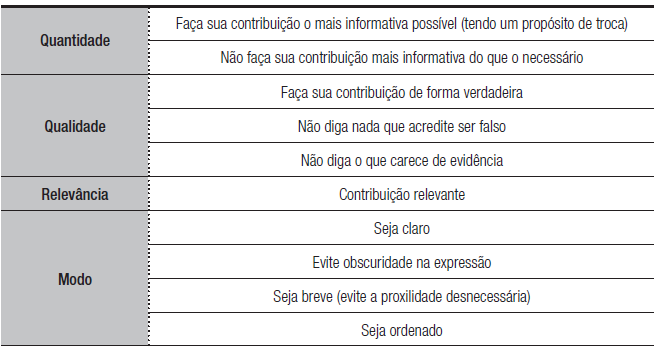
\includegraphics[width=1.0\textwidth]{./dados/figuras/distribuicao-grice}
	\fonte{\citeonline{Greef2014}}
	\label{fig:quadro-grice}
\end{figure}

A divisão no quadro é muito adequada para um contexto como o da construção de texto de forma colaborativa onde há a possibilidade de comentários de diversas pessoas, o que é um pouco diferente da proposta do projeto de traduções, porém, também e aplicável levando em conta que o responsável pela tradução deve seguir este mesmo princípio para produzir um texto que seja uma tradução adequada, mas, que também seja claro e de fácil entendimento, e o responsável pela validação das traduções também deve se limitar a garantir estas características, sem se envolver em “rodeios” que não contribuam para a democratização do conhecimento contido no documento traduzido.

\citeonline{Greef2014} ainda chamam a atenção para o risco de que de forma não intencional, as atitudes de algum participante do processo possa produzir problemas em relação aos outros. Um exemplo poderia ser a não aprovação de uma tradução ou uma crítica a algum problema encontrado em uma tradução já realizada.

O resultado desta pesquisa pode promover um incentivo à comunidade acadêmica para se envolver na redução da barreira linguística e facilitar o acesso a informação.

         % Revisão de Literatura
% METODOLOGIA------------------------------------------------------------------

\chapter{METODOLOGIA}
\label{chap:metodologia}
O estudo que será feito é de natureza aplicada analítica e possui abordagem quantitativa e qualitativa em diferentes questões.

\section{DELINEAMENTO DA PESQUISA}
\label{sec:MetDelPesq}
A pesquisa se limita à produção de um indicador capaz de representar a disposição dos indivíduos e instituições consultados em colaborar com a criação do sistema de traduções.

\section{COLETA DE DADOS}
\label{sec:MetColDad}
A coleta de dados será realizada através de um questionário elaborado no Google Formulários (disponível no link: https://goo.gl/forms/MMJOHtpqXLWpit3p2), que apresenta questões diferentes para três perfis de pessoas: Estudante do ensino superior, Representante ou funcionário de uma instituição de ensino superior, Outro perfil. Como cada perfil dentre estes tem uma função diferente em relação à vivência acadêmica e desempenhariam funções diferentes no sistema proposto, caso seja implementado, achou-se conveniente elaborar questões personalizadas para cada perfil consultado.

\section{TRATAMENTO DE DADOS}
\label{sec:MetTratDad}
O Google Formulários apresenta, muito intuitivamente, as respostas de uma pesquisa e também produz uma planilha contento todas as respostas em formato CSV (Valores Separados por Virgula), o que facilita a mineração de outros dados, caso seja necessário. Sobre os resultados obtidos pode-se trabalhar com ferramentas de avaliação estatística disponíveis em linguagens de programação que são fortemente aplicadas a este fim como R e Python.
                   % Metodologia
% RESULTADOS-------------------------------------------------------------------

\chapter{CRONOGRAMA DE ATIVIDADES}
\label{chap:cronograma}

A execução deste projeto prevê as seguintes etapas:
\begin{itemize}
	\item ETAPA 1 - Levantamento bibliográfico: Nesta etapa serão pesquisados trabalhos científicos que tratem sobre produção colaborativa, onde não há exatamente um responsável pela produção de conteúdo, mas, uma colaboração de indivíduos e/ou instituições em prol de alguma causa ou objetivo. Será executada no primeiro mês.
	
	\item ETAPA 2 - Elaboração do questionário de pesquisa: Esta etapa compreende a elaboração das questões que comporão o questionário que será utilizado para a coleta de dados do trabalho. Será executada no primeiro mês.
	
	\item ETAPA 3 - Elaboração do projeto de pesquisa: Esta etapa compreende a elaboração do presente projeto de pesquisa que orientará toda a execução do estudo. Será executada no primeiro mês
	
	\item ETAPA 4 - Coleta de dados: Nesta etapa o questionário de pesquisa será divulgado para o máximo de pessoas possível de forma orgânica (cada pessoa apresenta o questionário a conhecidos) para obter-se a maior massa de dados possível com o menor custo possível. Será executada durante o segundo e terceiro mês.
	
	\item ETAPA 5 - Analise dos dados: Nesta etapa, os dados obtidos pelo questionário de pesquisa serão tratados pra obter-se um indicador confiável sobre a disposição de instituições e alunos em colaborar com a plataforma colaborativa sugerida. Será executada no quarto mês.
	
	\item ETAPA 6 - Elaboração do relatório final: Nesta etapa, as informações obtidas no tratamento dos dados serão reunidas às obtidas na pesquisa bibliográfica e organizadas para a melhor compreensão possível. Será executada no quinto mês.
	
	\item ETAPA 7 - Revisão do texto: Nesta etapa o texto produzido na etapa anterior será revisado não só quanto à ortografia, mas, também aderência ao modelo exigido e à semântica das informações apresentadas. Será executada no sexto mês.
	
	\item ETAPA 8 - Entrega do trabalho: Nesta etapa será realizada a entrega do trabalho e sua apresentação. Será realizada no fina do sexto mês.
\end{itemize}

\begin{table}[!htb]
    \centering
    \caption[Tabela de atividades]{Tabela de atividades.
    \label{tab:tabela-exemplo1}}
    \begin{tabular}{|c|c|c|c|c|c|c|}
    	\hline
    	Atividade & 1º Mês & 2º Mês & 3º Mês & 4º Mês & 5º Mês & 6º Mês \\ \hline
    	Etapa 1 & X &   &   &   &   &   \\ \hline
    	Etapa 2 & X &   &   &   &   &   \\ \hline
    	Etapa 3 & X &   &   &   &   &   \\ \hline
    	Etapa 4 &   & X & X &   &   &   \\ \hline
    	Etapa 5 &   &   &   & X &   &   \\ \hline
    	Etapa 6 &   &   &   &   & X &   \\ \hline
    	Etapa 7 &   &   &   &   &   & X \\ \hline
    	Etapa 8 &   &   &   &   &   & X \\ \hline
    \end{tabular}
    \fonte{O autor}
\end{table}
                    % Cronograa de Atividades

\postextual
% INSERE ELEMENTOS PÓS-TEXTUAIS
% REFERÊNCIAS------------------------------------------------------------------

% Carrega o arquivo "base-referencias.bib" e extrai automaticamente as referências citadas

\bibliography{./base-referencias}
\bibliographystyle{abntex2-alf} % Define o estilo ABNT para formatar a lista de referências
% OBSERVAÇÕES------------------------------------------------------------------
% Este arquivo não precisa ser alterado.
           			   % Referências

\end{document}
